\documentclass[12pt,a4paper]{article}
\usepackage[utf8]{inputenc}
\usepackage{amsmath}
\usepackage{graphicx}
\usepackage{physics}
\usepackage{listings} 



\title{Computational Physics -- Problem Set 1}
\author{Tony Liu B05202068}


\begin{document}
    \maketitle

\section{Machine Precision}%
\label{sec:machine_precision}

    In my platform(Ubuntu 19.04), the smallest difference between two numbers that the computer can recognizes is the following. For the single precision, when $\epsilon$ is less then $5.9604644775390625\times 10^{-8} $, the error is negligible. For the double precision, when $\epsilon$ is less than  $1.11022302462515654042 \times 10^{-16}$, the error is negligible. The exponent in the case of double precision is two times larger than the exponent in the case of single precision.

\begin{align*}
    \alpha &= aldkjf\\
\beta &= aldskfaj
\end{align*}
    

\section{Richarsion Extrapolation}%
\label{sec:richarsion_extrapolation}

    
The second derivative of $f(x) = xe^{x}$ at $x = 2$, by using 3-point formula  \[
        f^{\prime \prime}(x) = \frac{f(x+h)-2f(x)+f(x-h)}{h^2}
    .\]
The Richardson extrapolation: 
\[
f^{\prime \prime}(x) &= D_{1}(h) \equiv \frac{f(x+h)-2f(x)+f(x-h)}{h^2} + O(h^2).
\]        
\[
        f^{\prime \prime}(x) &= D_{1}\Big(\frac{h}{2}\Big) \equiv \frac{f(x+\frac{h}{2})-2f(x)+f(x-\frac{h}{2})}{\frac{h^2}{4}} + O(\frac{h^2}{4}).
\]     
\begin{multline*}
    \Rightarrow D_{2}\Big(\frac{h}{2}\Big) \equiv  \frac{4D_{1}(\frac{h}{2}) - D_{1}(h)}{4-1} &= \frac{16f(x+ \frac{h}{2})-f(x+h) - 30f(x) +16f(x-\frac{h}{2})-f(x-h)}{3h^2} + O(\frac{h^{4}}{16})   
\end{multline*}
Similarly, to obtain $D_{3}\Big( \frac{h}{4}\Big)$, one computes 
\[
    D_{1}\Big(\frac{h}{4}\Big) = \frac{f(x+\frac{h}{4})-2f(x)+f(x-\frac{h}{4})}{(\frac{h}{4})^2} + O(\frac{h^2}{16})
.\]

\[
\Rightarrow D_{2}\Big(\frac{h}{4}\Big) = \frac{4D_{1}(\frac{h}{4}) - D_{1}(\frac{h}{2})}{4-1}  + O (\Big(\frac{h}{4}\Big)^{4}) 
.\]
Therefore,
\[
D_{3}\Big( \frac{h}{4}\Big) = \frac{4^2D_{2}(\frac{h}{4}) - D_{2}(\frac{h}{2})}{4^2 - 1} + O(\Big(  \frac{h}{4}\Big)^{6})
.\]
In general, for every iteration step $i$, 
\[
D_{i+1}\Big(\frac{h}{2}\Big) = \frac{4^{i}D_{i}(\frac{h}{2}) - D_{i}(h)}{4^{i} - 1}
.\]

From the C code, $f^{\prime \prime}(2)$ is obtained in the various precision shown below:
\begin{center}
\begin{tabular}{c   c   c   c   c   c}
    \centering
    $h$   &   $D_{1}$       &   $D_{2}$     &   $D_{3}$     &   $D_{4}$     & $D_{5}$     \\ \\
    0.4   &30.1515674803\\ 
    0.2   &29.7042684744    & 29.5551688058\\
    0.1   &29.5931861000    &29.5561586419  &29.5562246310\\
    0.05  &29.5654617422    &29.5562202895  &29.5562243994  &29.5562243957\\
    0.025 &29.5585335399    &29.5562241391  &29.5562243958  &29.5562243957  &29.5562243957\\
\end{tabular}
\end{center}

The exact solution for $f^{\prime \prime}(x)$ is 29.5562243957.\\
For $h = \frac{0.4}{2^{7}}, \frac{0.4}{2^{8}}, \frac{0.4}{2^{9}}, \frac{0.4}{2^{10}}$, I plot the values of the second derivative versus different iteration steps. As shown in the following figure, when the iteration steps increases, the values closely approache to the exact solution.


\begin{figure}[htpb]
    \centering
    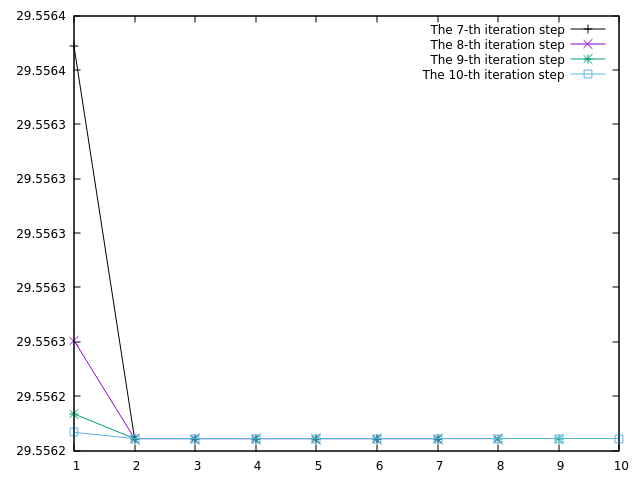
\includegraphics[width=0.8\linewidth]{Different Iteration Steps.png}
\end{figure}\\
\newpage

On the other hand, we can see that $D_{1}(h)$ decreases at the order of $h^{2}$ anad $D_{2}(h)$ decreases at the order of $h^{4}$. The plots below demonstrate this fact.\\
Below is the plot of $D_{1}(h) - f^{\prime \prime}(2)$ versus $h$ and the fitting function $g(x)$ is  $3.73618x^{2}-0.00638372x+7.15812\times 10^{-5}$\\
\begin{figure}[htpb]
    \centering
    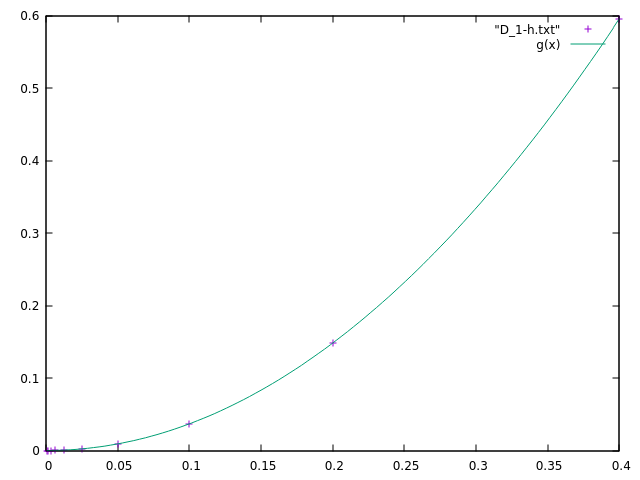
\includegraphics[width=0.5\linewidth]{D_1-h.png}
    \caption{D_1-H}%
    \label{fig:D_1-h}
\end{figure}\\

\newpage
Below is the plot of $D_{2}(h) - f^{\prime \prime}(2)$ versus $h$ and the fitting function $g(x)$ is  roughly $-0.0414696x^{4}+0.000115702x^{3}$

\begin{figure}[htpb]
    \centering
    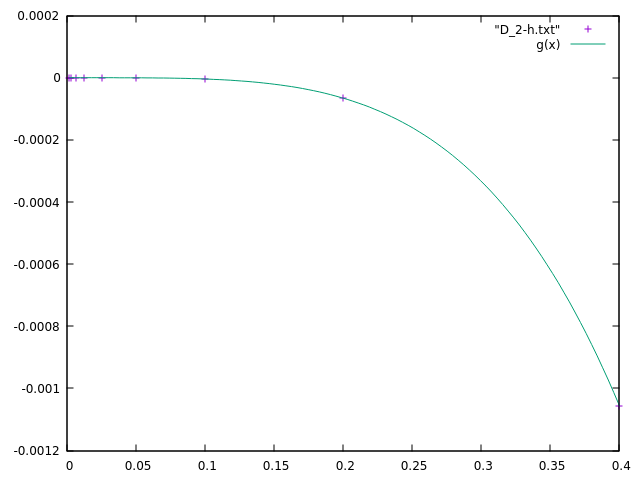
\includegraphics[width=0.5\linewidth]{D_2-h.png}
    \caption{D_2-H}%
    \label{fig:D_2-h}
\end{figure}

It is therefore expected that for $k >2$, $D _{k}(h)$ will decrease in the order of $h^{2k}$. Hence, the computed values will rapidly converge to the desired solution.
\end{document}
